\section{Описание решения}
В этой главе подробно рассмотрен весь алгоритм распознавания речевых команд. Для удобства понимая названия параграфов расположены в том же порядке, что и этапы в самом алгоритме.

\subsection{Предобработка}
Каждая команда записана в звуковой wav файл. В каждом файле - набор амплитудных значений, которые были получены в результате записи команд дикторами. 

\subsubsection{Нормализация сигнала}
В начале проводится нормализация амплитуд. Каждое значение амплитуды приводится к такому значению, чтобы минимум среди всех амплитуд звуковой дорожки был в 0, а максимум среди всех - в 1 по формуле:
\begin{equation}
	\overline{x}_i=\dfrac{x_i}{\max_{j} |x_j|},~i=\overline{0, p-1},~j \in [0, p-1]
\end{equation}
где $x$ - значение амплитуды, $\overline{x}$ - новое значение амплитуды, $p$ - количество амплитудных значений в звуковой дорожке.

Таким образом все значения амплитуд принимают значения в диапазоне $[0,1]$.

\subsubsection{Удаление постоянной составляющей}
Постоянная составляющая (DC-offset) - это смещение амплитуды сигнала на некоторую постоянную величину. Возникает это в аналого-цифровом сигнале из-за разницы напряжения между звуковой картой и устройством ввода. Данный эффект является помехой, от которой нужно избавиться. Для этого необходимо вычесть из каждого значения амплитуды среднее арифметическое всех значений амплитуд по формуле:
\begin{equation}
\overline{x}_i=x_i - \sum_{j=0}^{p-1} x_j,~i=\overline{0, p-1}
\end{equation}
где $x$ - значение амплитуды полученное на этапе нормализации, $\overline{x}$ - новое значение амплитуды, $p$ - количество амплитудных значений в звуковой дорожке.

\subsubsection{Выделение начальной и конечной точек слова}
Каждая звуковая дорожка содержит в себе помимо фрагментов звукового сигнала - команды ещё и фрагменты тишины. Очень важно отделить звуковой сигнал от фрагментов тишины, т. к. именно он несёт в себе всю информацию о команде. 

Для того, чтобы выделить звуковой сигнал и <<обрезать>> тишину в начале и в конце записи, используется алгоритм, описанный статье \cite{SignalPreprocessing}. 
Каждая звуковая дорожка разбивается на фреймы - наборы амплитуд, каждый длительностью 20 мс. Начала фреймов расположены с периодичностью 10 мс. Таким образом, фреймы пересекаются между собой. Это обеспечивает целостность обработки звукового сигнала, т.е. позволяет не упустить важные фонемообразующие особенности.

Затем для каждого фрейма вычисляется мгновенная энергия:
\begin{equation}
E_k = \sum_{m=0}^{N-1} x_{k_m}^2,~k=\overline{0,z-1}
\end{equation}
где $z$ - количество фреймов для конкретной звуковой записи, N - длина одного фрейма (количество амплитуд в одном фрейме).

Мгновенная энергия имеет один значительный недостаток. У неё очень большая чувствительность к относительно большим значениям амплитуды из-за возведения во вторую степень. Это ведёт к искажению соотношений отсчётов звукового сигнала между друг другом. Поэтому функция мгновенной энергии переопределяется как:
\begin{equation}
\label{eq:instant_energy}
E_k = \sum_{m=0}^{N-1} |x_{k_m}|,~k=\overline{0,z-1}
\end{equation}

После того, как посчитаны мгновенные энергии для каждого фрейма, вычисляется нижнее и верхнее пороговые значения:
\begin{equation}
\begin{aligned}
& I_1 = 0.03 \cdot (MX - MN) + MN \\
& I_2 = 4 \cdot MN \\
& ITL = min(I_1,~I_2)\\
& ITU = 10 \cdot ITL
\end{aligned}
\end{equation}
где $MN$, $MX$ - минимум и максимум мгновенной энергии среди всех фреймов соответственно, $ITL$, $ITU$ - нижнее и верхнее пороговое значение.

Происходит поиск фрейма, с которого начинается слово с самого первого фрейма. Фрейм, в котором значение мгновенной энергии превышает $ITL$, предварительно помечается как начало слова. Затем начиная с этого помеченного фрейма происходит поиск фрейма, в котором значение мгновенной энергии превышает $ITU$. Если значение мгновенной энергии для какого-то фрейма во время последнего поиска меньше $ITL$, то этот фрейм становится предварительным началом слова. 

Аналогично происходит поиск конца слова в звуковой дорожке. Только поиск по фреймам происходит не с начала сигнала, а с конца.

После этого этапа имеются два предварительно помеченных фрейма $m_{begin}, m_{end}$  - начало и конец слова в звуковом файле.

Функция мгновенной энергии, определённая формулой \eqref{eq:instant_energy} хорошо справляется с отделением звонких звуков от тишины. Но вот глухие она отделяет плохо. Поэтому используется вторая характеристика для доопределения начала и конца слова - число переходов через ноль. Это количество таких случаев, когда соседние отсчёты (значения амплитуд) имеют противоположные знаки. Определяется формулой:
\begin{equation}
	Z_k = \dfrac{1}{2} \sum_{m=1}^{N-1} |sgn(x_{k_{m-1}}) - sgn(x_{k_m})|,~k=\overline{0,z-1}
\end{equation}
Подразумевается, что первые 100 мс звуковой записи - это тишина, и речь начинается позднее.

Вычисляется среднее значение переходов через ноль в течение первых 100 мс \eqref{eq:izc},  среднее квадратическое отклонение количества переходов через ноль в течение первых 100 мс \eqref{eq:deviation}:
\begin{align}
	\label{eq:izc}
	&IZC = \dfrac{1}{z} \sum_{k=0}^{z-1} Z_k \\
	\label{eq:deviation}
	&\sigma_{IZC} = \sqrt{\dfrac{1}{z} \sum_{k=0}^{z-1} (Z_k - IZC)^2}
\end{align}
а затем пороговую функцию числа переходов через ноль по формуле:
\begin{equation}
	IZCT = min(IF,~IZC + 2 \sigma_{IZC}),
\end{equation}
где $IF$ - фиксированное количество переходов через ноль. В данном случае 
то 25 пересечений за 10 мс, то есть $IF=2.5$. 

Происходит уточнение точек начала и конца слова в звуковой дорожке. Начиная от фрейма $m_{begin}$ влево происходит поиск фреймов, у которых число переходов через ноль выше порогового значения. Поиск происходит всего на расстоянии 25 фреймов, так как производится уточнение границ слова. Если пороговое значение было превышено 3 или более раз, то фрейм $r_{begin}$, где это произошло впервые, помечается как начало слова. Иначе метка $m_{begin}$ переобозначается как $r_{begin}$.

Аналогично от фрейма $m_{end}$ происходит поиск вправо для уточнения точки конца слова, которая обозначается за $r_{end}$.

В результате имеется 2 помеченных фрейма - $r_{begin}, r_{end}$. Сигнал обрезается, и в нем остаётся только речевая команда в виде набора фреймов $[r_{begin}, ... , r_{end}]$. Обозначим количество получившихся фреймов за $u$ и пронумеруем фреймы следующим образом: $[r_0, ... , r_{u-1}]$.

\subsection{Выделение речевых признаков}
Для того, чтобы выделить речевые признаки, используется алгоритм MFCC \cite{MFCC}. Он является одним из стандартных подходов к решению поставленной задачи. Состоит MFCC из нескольких шагов:
\begin{enumerate}
	\item Для каждой звукового сигнала проделать шаги:
	\begin{enumerate}
		\item Разбить сигнал на фреймы.
		\item Для каждого фрейма проделать шаги:
		\begin{enumerate}
			\item Получить спектр сигнала.
			\item Составить набор мел-фильтров в соответствии с оконной функцией.
			\item Применить мел-фильтры к спектру сигнала.
			\item Прологарифмировать результат, полученный на предыдущем шаге.
			\item Применить дискретное косинусное преобразование к результату предыдущего шага.
		\end{enumerate}
		\item Объединить MFCC векторы коэффициентов в матрицу.
	\end{enumerate}

	\item Привести матрицы коэффициентов MFCC каждой звуковой дорожки к одной размерности. Для этого дополнить их нулями слева до необходимой длины. Унифицированная размерность матриц выбирается как максимальная среди всех.
\end{enumerate}
  
Так как на выходе алгоритма выделения начальной и конечной точек слова получается набор фреймов, то шаг разбиения сигнала на фреймы опускается.

\subsubsection{Получение спектра сигнала}
Спектр сигнала $S_{k_m}$ в $k$-ом фрейме - результат дискретного преобразования Фурье:
\begin{equation}
	S_{k_m} = \sum_{n=0}^{N-1} x_{k_n} \cdot e^{\dfrac{-2\pi i}{N}mn},~m=\overline{0,N-1},~k=\overline{0,u-1}
\end{equation}

\subsubsection{Мел-шкала и расчёт мел-фильтров}
Мел - психофизическая единица высоты звука. Она описывает значимость конкретной частоты в человеческом восприятии. 
Популярные формулы для перевода Герц в 
Мел и обратно описаны в книге \cite{Mel} на стр. 150:
\begin{align}
	&mel(hz) = 1127 \cdot ln(1 + \dfrac{hz}{700})\\
	&hz(mel) = 700 \cdot (e^{\dfrac{mel}{1127}}-1)
\end{align}

На рисунке \ref{fig:hz_mel} изображено сравнение шкал Мел и Гц.

\begin{figure}[H]
	\[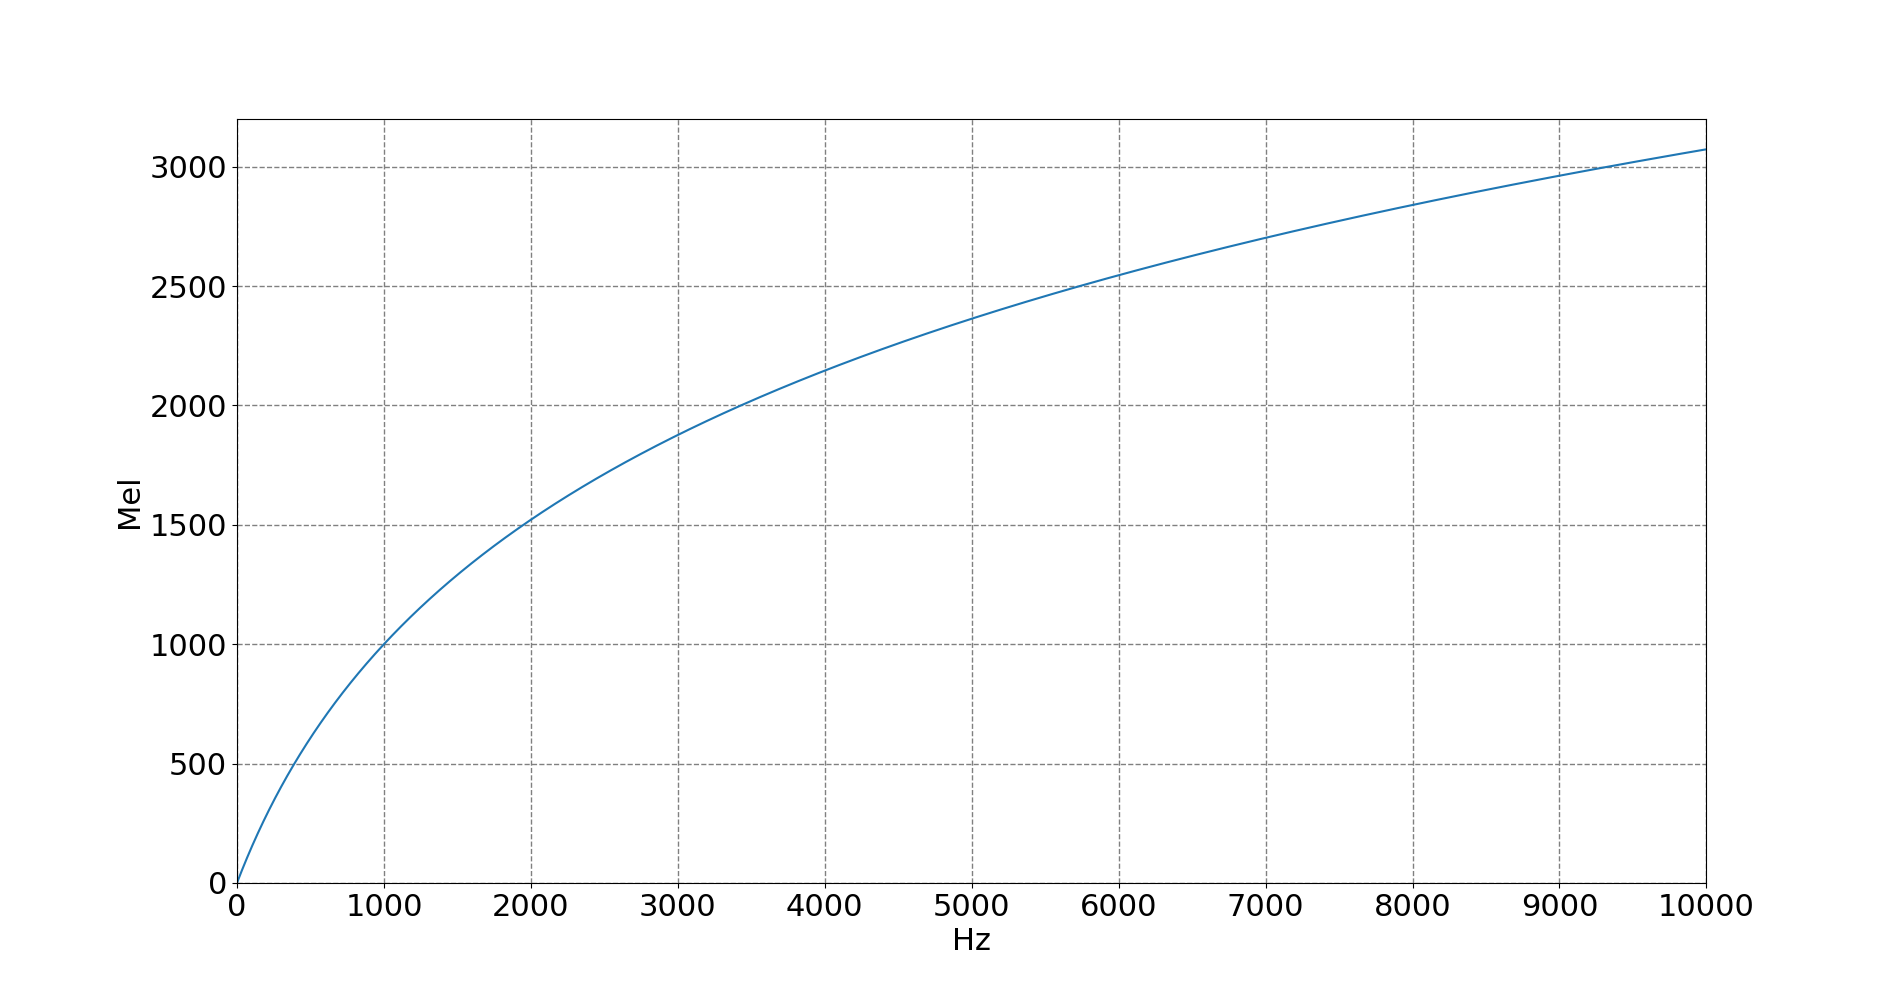
\includegraphics[scale=0.3]{hz_mel.png}\]
	\caption{Сравнение шкал Мел и Гц}
	\label{fig:hz_mel}
\end{figure}


Составляются треугольные Мел-фильтры в виде оконной функции:
\begin{equation}
	H(v,~b)=
	\begin{cases}
		0, 										     & \Phantom \phantom{-}    b < f(v)\\
		\dfrac{b-f(v)}{f(v+1)-f(v)},   & \Phantom f(v) \leq b \leq f(v+1)\\
		\dfrac{f(v+2)-b}{f(v+2)-f(v+1)}, & \Phantom f(v+1) \leq b \leq f(v+2)\\
		0,                                           & \Phantom \phantom{-}   b > f(v+2)\\
	\end{cases}
\end{equation}
для которой $f$ определяется как:
\begin{equation}
	f(a)=\dfrac{N}{w} hz(mel(f_{min})+a \dfrac{mel(f_{max})-mel(f_{min})}{Q+1}),
\end{equation}
где $w$ - частота дискретизации звуковой дорожки, $Q$ - количество треугольных мел-фильтров, $f_{min},~f_{max}$ - нижний и верхний пороги частотного диапазона соответственно, $m=\overline{0,N-1}$. Q обычно выбирается в диапазоне 20-40 (26 является своеобразным стандартом).

На рисунке \ref{fig:filters} в качестве примера изображена оконная функция для звуковой дорожки с параметрами $w=44100$ Гц, $f_{min}=0$ Гц, $f_{max}=22050$ Гц, $N=1024$, $Q=13$.

\begin{figure}[H]
	\[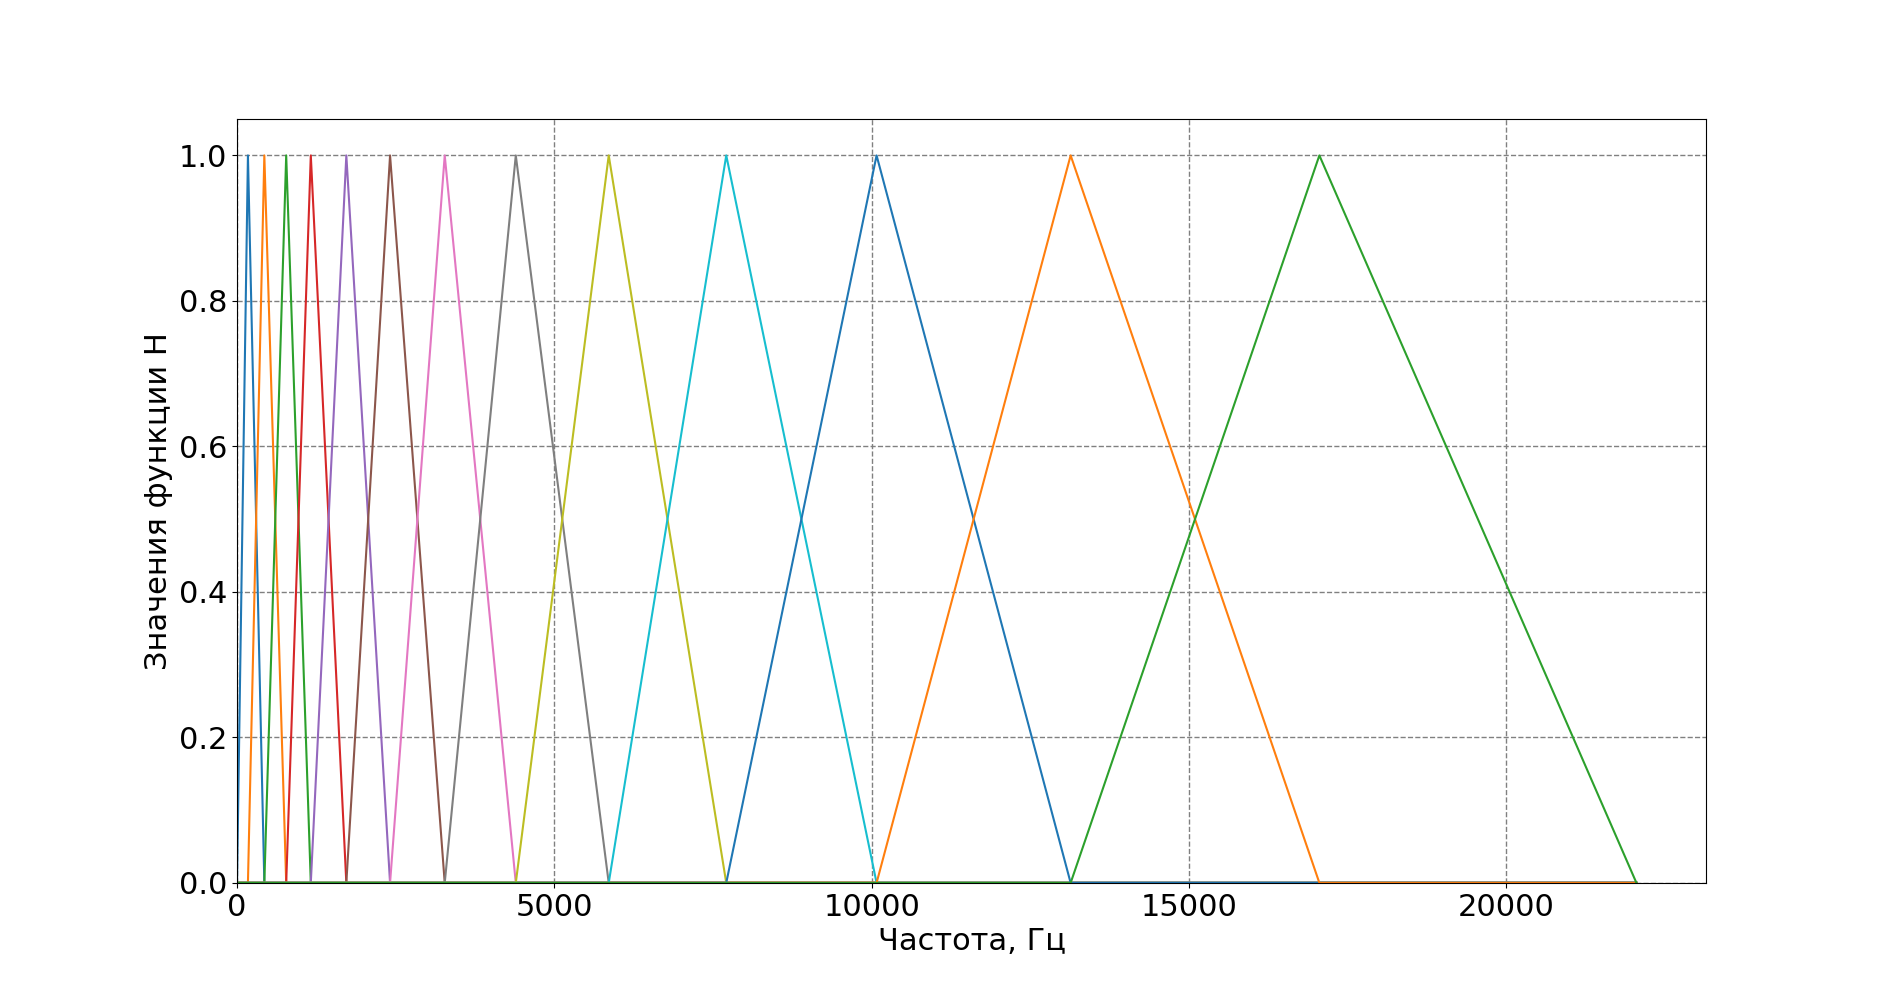
\includegraphics[scale=0.3]{filters.png}\]
	\caption{Оконная функция}
	\label{fig:filters}
\end{figure}

\subsubsection{Получение кепстра сигнала}
Кепстр -  определяется в виде обратного преобразования Фурье от логарифма спектра мощности сигнала:
\begin{equation}
	C(x(t))=F^{-1}(ln[F(x[t])])
\end{equation}
где $x(t)$ - входной сигнал, $F,~F^{-1}$ - прямое и обратное преобразование Фурье соответственно.

Кепстр совместно с мел-фильтрами используется для выделения речевых признаков. Эта та часть звукового сигнала, которая была образована при помощи голосового тракта человека. В книге \cite{CeptrumExplanation} можно найти описание того, как это происходит на стр. 367-380. 

Выше описан кепстр для непрерывного сигнала. В случае с дискретным набором амплитуд в сигнале и учитывая мел-фильтры, $ln[F(x[t])$ записывается как:
\begin{equation}
	W_{k_q} = ln(\sum_{m=0}^{N-1} |S_{k_m}|^2 \cdot H(q,m)),~q=\overline{0,Q-1},~k=\overline{0,u-1}
\end{equation}

В качестве обратного преобразования Фурье в алгоритме MFCC используется дискретное косинусное преобразование. Получение итоговых коэффициентов MFCC происходит по формуле:
\begin{equation}
	c_{k_n} = ln(\sum_{m=0}^{Q-1} W_{k_m} cos(\dfrac{\pi}{Q} (m+\dfrac{1}{2})n)),~n=\overline{0,d-1},d \le Q,~k=\overline{0,u-1},
\end{equation}
где $d$ - желаемое количество коэффициентов MFCC.

Таким образом получается матрица для каждой звуковой дорожки следующего вида:

\begin{equation*}
	C_{u \times d} = \left(
	\begin{array}{cccc}
		c_{00} & c_{01} & \ldots & c_{0(d-1)}\\
		c_{10} &  c_{11} & \ldots & c_{1(d-1)}\\
		\vdots & \vdots & \ddots & \vdots\\
		c_{(u-1)0} & c_{(u-1)1} & \ldots & c_{(u-1)(d-1)}
	\end{array}
	\right)
\end{equation*}
где $u$ - количество фреймов, получившееся после выделения начальной и конечной точек слова, $d$ - выбранное количество MFCC коэффициентов.

\subsubsection{Приведение данных к одной размерности}
Среди всех значений $u$ существует максимальное $u_{max}$. Для каждой матрицы, соответствующей определённой звуковой дорожке, проделаем следующее:
\begin{itemize}[leftmargin=2cm]
	\item если $u < u_{max}$, то соответствующая матрица $C$ дополняется нулями слева:
	\begin{equation*}
		C_{u_{max} \times d} = \left(
		\begin{array}{ccccccc}
			0 & \ldots & 0 & c_{00} & c_{01} & \ldots & c_{0(d-1)}\\
			0 & \ldots & 0 & c_{10} &  c_{11} & \ldots & c_{1(d-1)}\\
			\vdots & \ddots & \vdots & \vdots & \vdots & \ddots & \vdots\\
			0 & \ldots & 0 & c_{(u-1)0} & c_{(u-1)1} & \ldots & c_{(u-1)(d-1)}
		\end{array}
		\right)
	\end{equation*}
	\item если $u = u_{max}$, то матрица $C$ остаётся без изменений.
\end{itemize}

Таким образом, все матрицы приводятся к одной размерности $u_{max} \times d$.

\subsubsection{Сохранение данных}
\label{par:saving_preprocessed_data}
Матрицы коэффициентов объединяются в массив и записываются в файл <<speaker\{i\}\_data.npy>>\footnotemark \space в виде numpy массива. $i=\overline{1,6}$ здесь - номер диктора. В файл <<speaker\{i\}\_labels.npy>>\footnotemark[\value{footnote}] записываются индексы команд, в виде массива, в том же порядке, что и соответствующие им матрицы коэффициентов MFCC. Соответствие произнесённых диктором команд и их индексов представлено в таблице \ref{table:commands}.
 
\footnotetext{Фигурные скобки не являются частью имени файла}
 
\begin{table}[H]
	\small
 	\centering
	\csvautotabular{csv/commands.csv}
	\caption{Соответствие команд и их индексов}
 	\label{table:commands}
\end{table}

\subsection{Распознавание речевых команд}
Распознавание речевых команд происходит при помощи применения технологии нейронных сетей. В данной работе рассматриваются два типа нейронных сетей: многослойный персептрон и свёрточная сеть. Производится сравнение производительности этих двух типов при разных параметрах обучения.
\subsubsection{Многослойный персептрон}
Этот вид нейронной сети описан в третьей части книги Фрэнка Розенблатта \cite{Perceptron}, который первый предложил модель персептрона. Одним из достоинств многослойного персептрона является то, что это самая простая разновидность нейронной сети. Она состоит их входного слоя, полносвязных слоев и выходного слоя.
\subsubsection{Свёрточная нейронная сеть}
Данный тип нейронной сети был предложен Яном ЛеКуном \cite{CNN}. Это многослойная сеть, позволяющая обеспечить устойчивость распознавания к инвариантным изменениям данных за счёт общих весов и локального рецептивного поля.

Входной слой сети состоит из одной плоскости. Его размерность совпадает с размерностью входных данных. 

Последующие слои - свёрточные. Каждый свёрточный слой состоит из нескольких плоскостей нейронов, которые известны как карты признаков. Каждый нейрон в свёрточном слое соединён с небольшой областью предыдущего слоя. В этом заключается принцип локального рецептивного поля.

После каждого свёрточного слоя, который получил локальные признаки, стоит пулинг слой. Его задача состоит в понижении размерности данных.

После всех свёрточных слоёв следует выпрямляющий слой, который преобразует данные к вектору. 

Далее следуют полносвязные слои. Иногда добавляется дропаут слой, который отключает некоторые нейроны на разных эпохах обучения. Это позволяет бороться с переобучением сети.

Выходной слой имеет размерность требуемых выходных данных. 

\subsubsection{Входные и выходные данные модели}
Входной тензор модели - матрица MFCC коэффициентов для соответствующей команды. Его размерность - $u_{max} \times d$. Для составленного датасета $u_max=400, d=13$.
Выходной тензор имеет размерность $g \times 1$, где $g$ - количество возможных команд для распознавания. Для составленного датасета $g=11$. Индекс распознанной команды соответствует индексу максимального элемента выходного тензора. Индексация в тензоре начинается с 0.
\subsubsection{Архитектура нейронной сети}
Архитектура свёрточной нейронной сети приведена на рисунке \ref{fig:cnn_model}. Как видно из рисунка, сеть включает в себя:
\begin{itemize}[leftmargin=2cm]
	\item Входной слой InputLayer (размерность входных данных - $400 \times 13$)
	\item Слой свёртки Conv2D (32 нейрона, размерность ядра сверки - $5 \times 5$, функция активации - ReLu)
	\item Слой пулинга AveragePooling2D (размерность пула - $2 \times 2$)
	\item Слой свёртки Conv2D (64 нейрона, размерность ядра сверки - $5 \times 5$, функция активации - ReLu)
	\item Слой пулинга AveragePooling2D (размерность пула - $2 \times 2$)
	\item Выпрямляющий слой Flatten
	\item Полносвязный слой Dense (128 нейронов, функция активации - ReLu)
	\item Слой дропаута Dropout (процент исключения случайных нейронов  - 30\%)
	\item Выходной полносвязный слой Dense (11 нейронов, функция активации - Softmax)
\end{itemize}

\begin{figure}[H]
	\[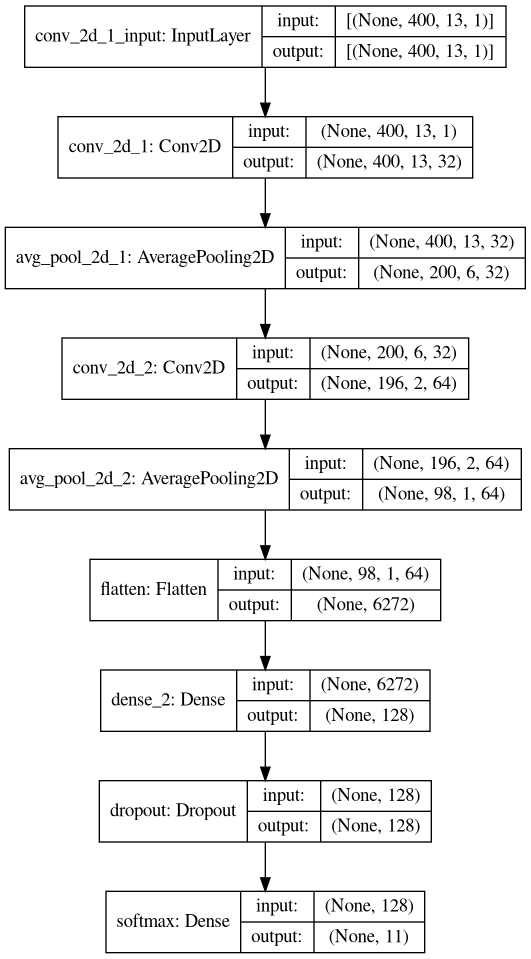
\includegraphics[scale=0.4]{cnn_model.png}\]
	\caption{Структура свёрточной нейронной сети}
	\label{fig:cnn_model}
\end{figure}

Архитектура свёрточной нейронной сети приведена на рисунке \ref{fig:cnn_model}. Как видно из рисунка, сеть включает в себя:
\begin{itemize}[leftmargin=2cm]
	\item Входной слой InputLayer (размерность входных данных - $400 \times 13$)
	\item Выпрямляющий слой Flatten
	\item Полносвязный слой Dense (256 нейронов, функция активации - ReLu, регуляризатор ядра - L2 c параметром $\lambda = 0.00001$)
	\item Полносвязный слой Dense (128 нейронов, функция активации - ReLu, регуляризатор ядра - L2 c параметром $\lambda = 0.00001$)
	\item Полносвязный слой Dense (128 нейронов, функция активации - ReLu, регуляризатор ядра - L2 c параметром $\lambda = 0.00001$)
	\item Полносвязный слой Dense (64 нейрона, функция активации - ReLu, регуляризатор ядра - L2 c параметром $\lambda = 0.00001$)
	\item Выходной полносвязный слой Dense(11 нейронов, функция активации - Softmax)
\end{itemize}

\begin{figure}[H]
	\[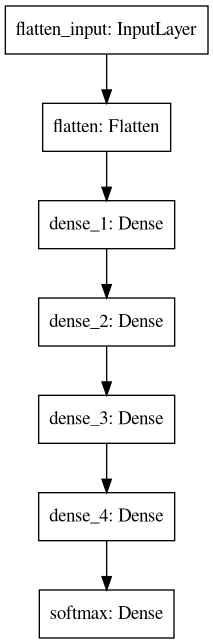
\includegraphics[scale=0.4]{mlp_model.png}\]
	\caption{Структура многослойного персептрона}
	\label{fig:cnn_model}
\end{figure}

\subsection{Программная реализация}
Построение программного интерфейса для блоков предобработки и распознавания команд было произведено при помощи языка программирования Python 3.8.

Блок предобработки был реализован при помощи библиотек numpy, scipy. 

Блок распознавания был реализован при помощи библиотек jupyterlab, Keras, numpy. Для анализа результатов обучения нейронных сетей были использованы библиотеки pandas, matplotlib, seaborn.

Программный комплекс разделен на две части:
\begin{itemize}[leftmargin=2cm]
	\item Корневой файл <<preprocessing.py>>, в котором реализована предобработка. Весь вспомогательный функционал вынесен в отдельный модуль <<helpers>>.
	\item Корневой файл <<boxy.ipynb>>, в котором реализовано обучение и тестирование нейронных сетей. Весь вспомогательный функционал также вынесен в отдельный модуль <<helpers>>.
\end{itemize}

В корневой директории <<recorded\_audio>> хранятся записанные шестью разными дикторами звуковые файлы, содержащие команды. Каждый файл содержит в своём названии индекс речевой команды, которая в нём записана.

В корневую директорию <<data>> в процессе предобработки файлов из директории <<recorded\_audio>> сохраняются файлы, описание которых приводится в разделе \ref{par:saving_preprocessed_data}:
\begin{itemize}[leftmargin=2cm]
	\item <<speaker\{i\}\_data.npy>>, $i=\overline{1,6}$ - номер диктора
	\item <<speaker\{i\}\_labels.npy>>, $i=\overline{1,6}$ - номер диктора.
\end{itemize}

В корневой директории <<logs>> в процессе предобработки данных создаётся файл <<log.log>>, в который записывается краткий отчёт об обработке каждой звукового файла.


Для создания датасета для обучения и тестирования нейронных сетей был разработан веб-сервис при помощи языков Javascript, HTML, CSS и фреймворка NodeJS. Этот сервис позволяет записывать речевые команды и сохранять их в нужном для программы предобработки wav формате с правильным названием. Это позволило в короткие сроки записать необходимое количество дикторов и уменьшило скорость записи в несколько раз, так как в обычных программах записи звука очень много времени уходит на сохранение с правильными параметрами. Ссылка на сервис и его код доступны в приложении.

\subsection{Описание датасета}
Составленный датасет состоит команд, записанных шестью дикторами. Каждый диктор работал с 11 командами : <<back>>, <<down>>, <<menu>>, <<off>>, <<on>>, <<open>>, <<play>>, <<power>>, <<stop>>, <<up>>, <<volume>>. В таблице \ref{table:dataset} указаны типы голосов дикторов и данные количестве записанных команд.


\begin{table}
\begin{tabular}[c]{ | p{1.8cm} | p{2cm} | p{5.8cm} | p{4cm} | }
	\hline
	Диктор & Тип голоса & Кол-во звук. дорожек на каждую команду & Сумм. кол-во звук. дорожек  \\ \hline
	speaker1 & Мужской & 50 & 550 \\
	speaker2 & Мужской & 40 & 440 \\
	speaker3 & Мужской & 40 & 440 \\
	speaker4 & Мужской & 40 & 440 \\
	speaker5 & Мужской & 50 & 550 \\
	speaker6 & Женский & 50 & 550 \\ \hline
	
\end{tabular}
\caption{\label{table:dataset}Типы дикторов и данные количестве записанных команд}
\end{table}

Датасет предварительно разделяется на тренировочную и тестовую части. На тренировочную часть отводится 70\% данных диктора, на тестовую часть - 30\%.
